\section{Design decisions}

\subsection{Database}
We use MongoDB for our database. We chose to use this database as it is easy to implement and easy to use. We have
a MongoDB database with 1 collection, Bikes. The Bikes collection stores all bike locations and their availability. There should be a second database collection, Users, for storing the name, passwords and a list of rented bikes. Due to lack of time, we weren't able to implement this correctly.  


    \begin{figure}[H]
		\centering
		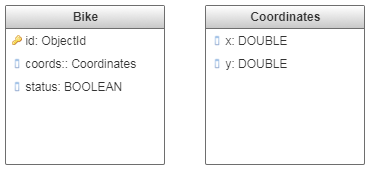
\includegraphics[width=0.3\textwidth]{images/db-structure.png}
		\caption{Overview of the database}
		\label{database}
	\end{figure}
	
	
\subsection{Webserver}
Why Play Framework with Scala

\subsection{Client}
Why Angular and Bootstrap
